\documentclass[10pt]{beamer}
\usepackage[utf8]{inputenc}
\usetheme{default}
\usecolortheme{dove}
\usepackage{textpos}
\usepackage{grid-system}
\usepackage[T1]{fontenc}

\AtBeginSection[]
{
  \begin{frame}<beamer>
    \frametitle{Übersicht}
    \tableofcontents[currentsection]
  \end{frame}
}

% TODO:
% - Hinweis auf Cryptoparty Computerwerk?
% - "Vision" aus 2015-10-04_VeganBrunch einarbeiten, wo sinnvoll
% - Welche Router kaufen?

% TODO: Vielleicht kann man die Titelfolie noch ein wenig aufpeppen?
% - Hintergrundbild?
% - Warum ist unser Footer mitten auf der Seite?
%   -> Footer ohne Logo nach unten
%   -> Großes Logo in die Mitte
\title{Freifunk Darmstadt}
\author{}
\institute[Inst.]{eine Initiative des Chaos Darmstadt e.V.}
\date{\footnotesize 20. Februar 2016}

\begin{document}
  \addtobeamertemplate{frametitle}{}{
    \begin{textblock*}{0cm}(\textwidth-0.85cm,-0.85cm)
      %
\includegraphics[height=1cm]{images/logo}
      \begin{figure}[h]
        \def\svgwidth{1.5cm}
        \input{logo.pdf_tex}
      \end{figure}

    \end{textblock*}
  }

  \begin{frame}
    \centering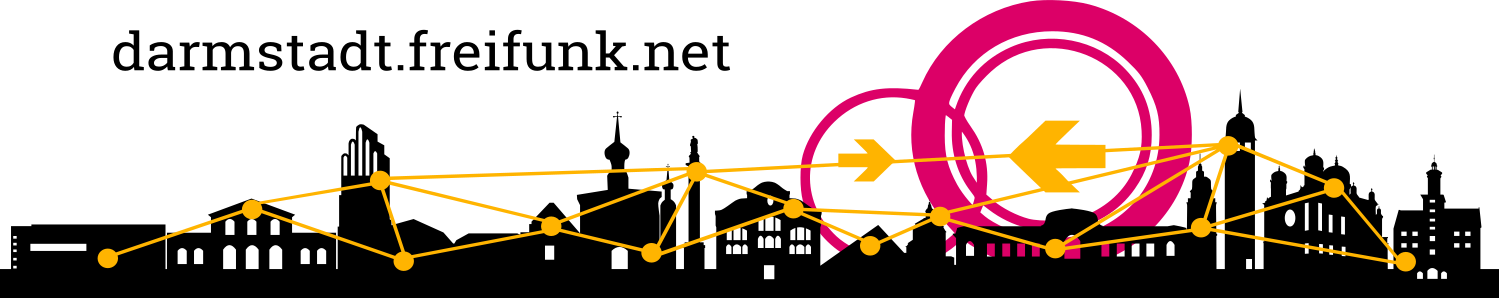
\includegraphics[width=\textwidth]{images/logo-skyline}
    \maketitle
  \end{frame}

  \begin{frame}{Übersicht}
    \tableofcontents
  \end{frame}

  \section{Was ist Freifunk?}

    \begin{frame}{Was ist Freifunk?}
      \large \textbf{Deutschlandweite Initiative für \emph{freie} Netze.}
      \begin{center}
        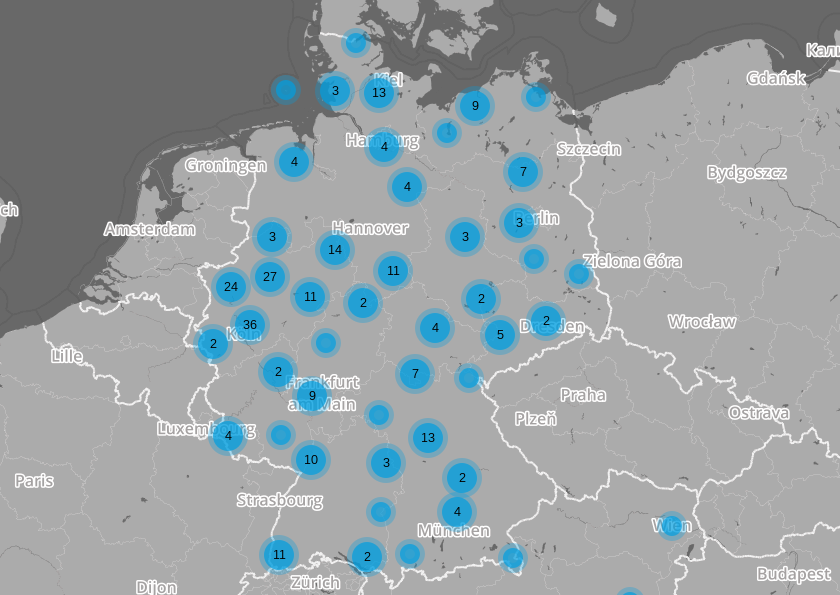
\includegraphics[height=12em]{images/2016-02-17_map-de}
      \end{center}
      \begin{itemize}
        \item 275 lokale Gruppen
        \item fast 30.000 offene Zugangspunkte\footnote{\url{http://freifunk.net/map/map.html}}
        \item Teil einer weltweiten Bewegung für offene und freie Netze
      \end{itemize}
    \end{frame}

    \begin{frame}{Prinzipien}
      \begin{centering}
        \large{\textbf{Wie sollte die Infrastruktur für unsere tägliche Kommunikation beschaffen sein?}}
      \end{centering}
      \vfill
      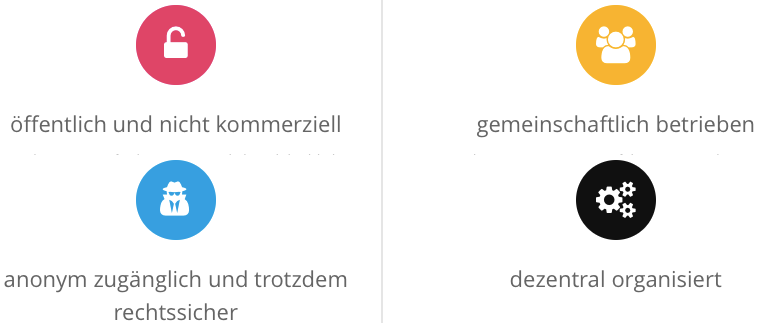
\includegraphics[width=1.1\textheight]{images/principles}

      % freie, ungehinderte Teilnahme an Betrieb und Ausbau des Netzes
      % Mitmachnetz
      % im Besitz der Gemeinschaft
      % anonymer, unzensierter Zugang zu Netz und Diensten
      % keine Unterscheidung} nach Ort oder Geldbeutel
      % Datensparsamkeit
      % Unterstützung jederzeit willkommen

    \end{frame}

    \begin{frame}{Ziele von Freifunk}
      \begin{columns}[T]
        \begin{column}{5cm}
          \begin{itemize}
            \item \textbf{Verständnis von Kommunikationsnetzen} sowie deren Auswirkungen auf die Gesellschaft fördern
            \item Teilnahme der Bevölkerung an \textbf{Forschung und Aufbau} dezentraler Netze
            \item unser \textbf{Wissen und Software} öffentlich zugänglich machen
            \item Beteiligung an politischen Prozessen, um \textbf{rechtliche Voraussetzungen} für freie Netze zu schaffen
          \end{itemize}
        \end{column}
        \begin{column}{5cm}
          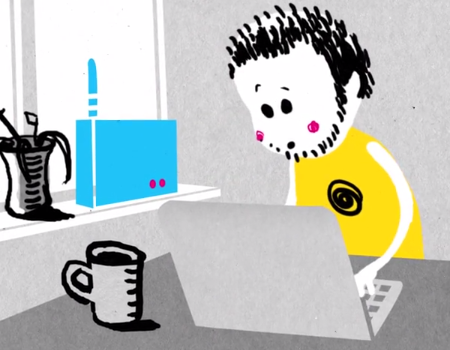
\includegraphics[width=0.9\textwidth]{images/install}
          \vspace{0.5em}
          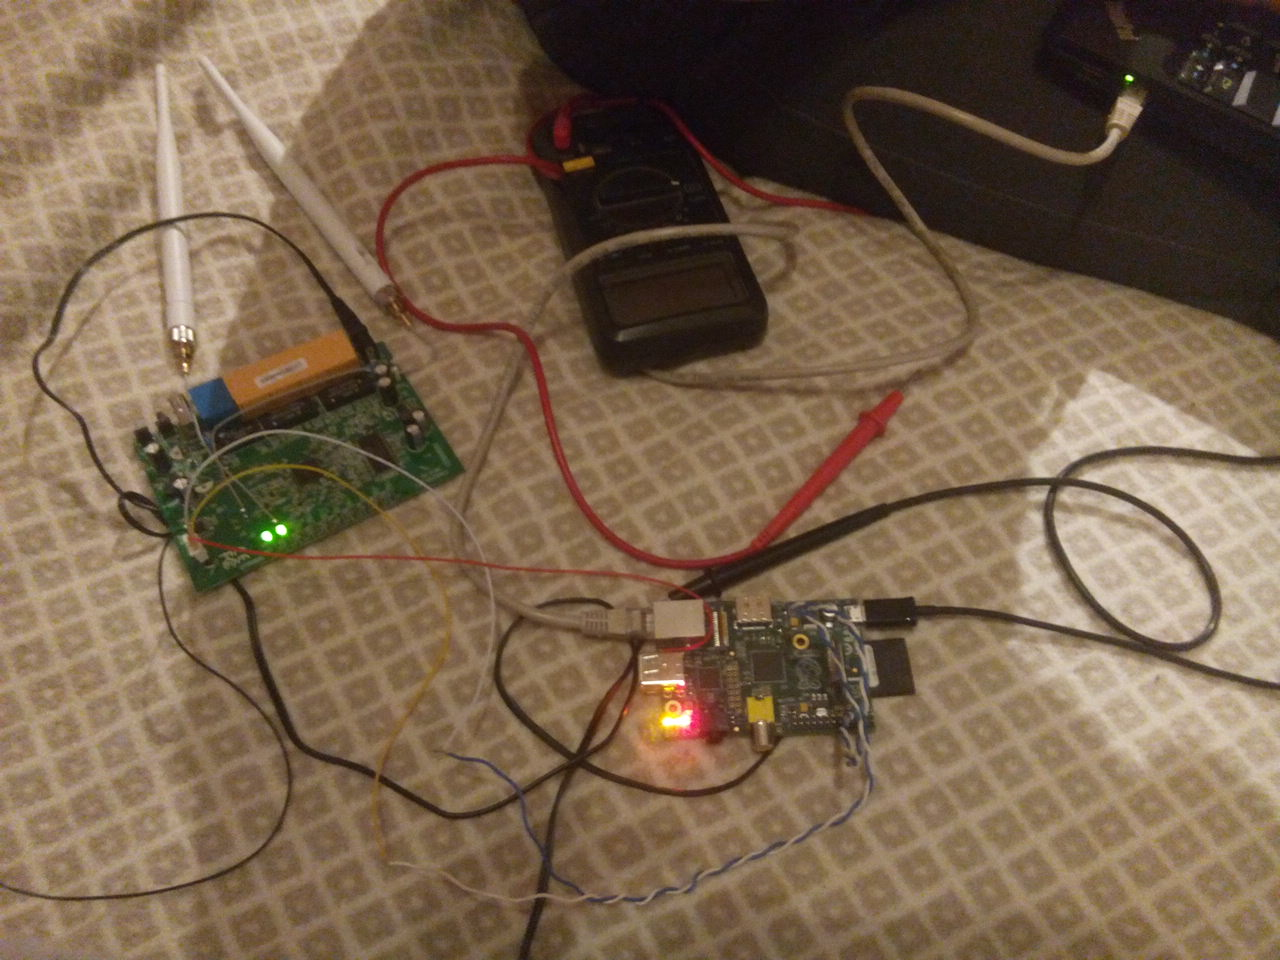
\includegraphics[width=0.9\textwidth]{images/disassemble}
        \end{column}
      \end{columns}
    \end{frame}

    \begin{frame}{Wie sieht so ein freies Netz aus?}
      \begin{center}
        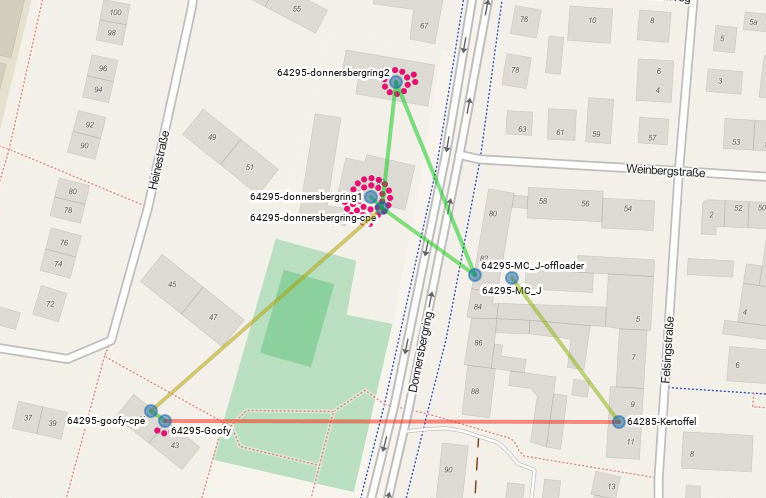
\includegraphics[height=6cm]{images/2016-02-17_donnersbergring}
        \vfill Donnersbergring
      \end{center}
    \end{frame}

    \begin{frame}{Wie sieht so ein freies Netz aus?}
      \begin{center}
        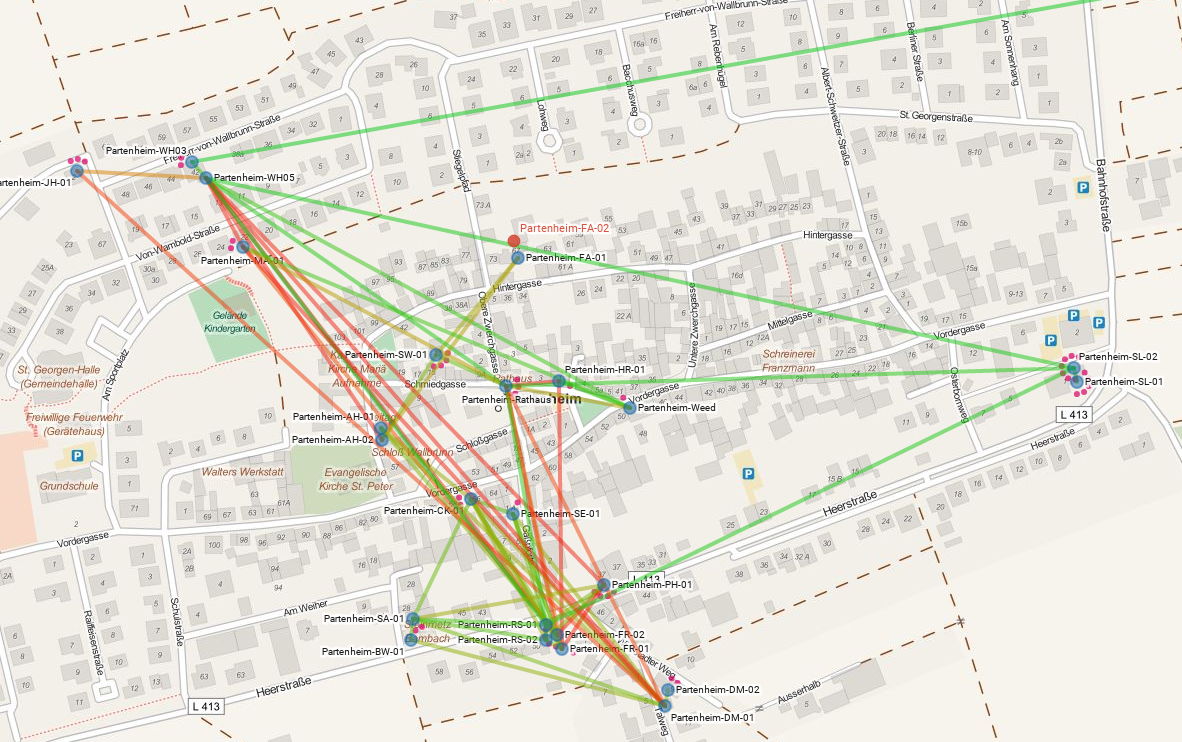
\includegraphics[height=6cm]{images/2015-10_partenheim-map}
        \vfill Partenheim bei Mainz
      \end{center}
    \end{frame}

    \begin{frame}{Wie sieht so ein freies Netz aus?}
      \begin{center}
        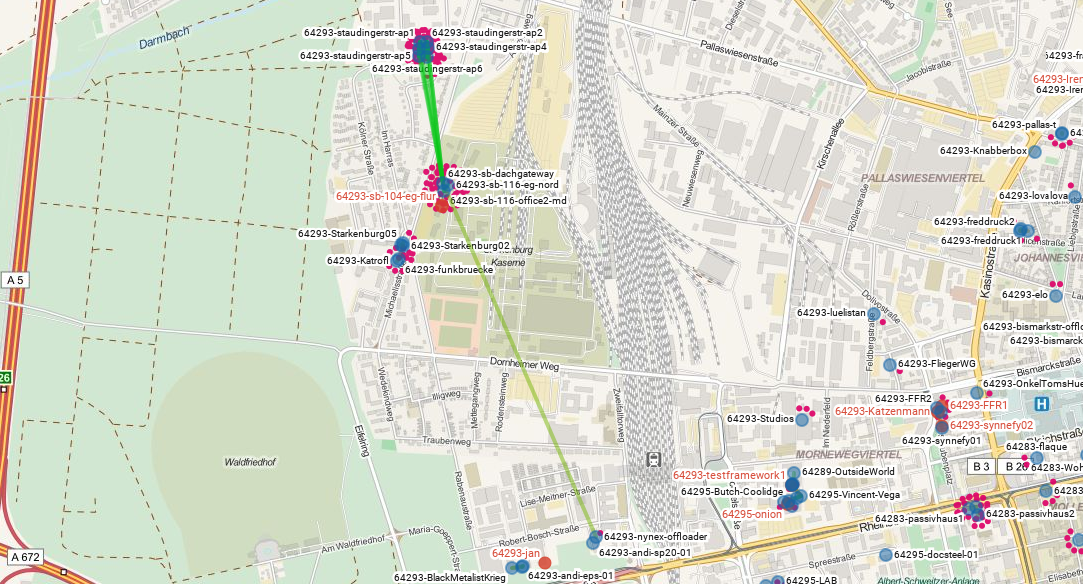
\includegraphics[height=6cm]{images/2016-02-17_starkenburk-link}
        \vfill Versorgung der Geflüchteten
        \vfill \small Starkenburgkaserne und Staudinger Straße
      \end{center}
    \end{frame}

    \begin{frame}{Warum ein freies Netz?}
      \vfill
      \begin{center}
        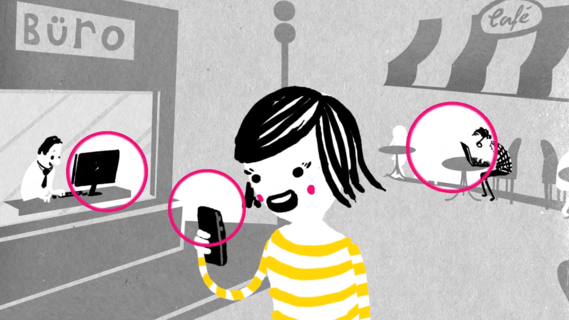
\includegraphics[width=5.5cm]{images/verbindet}
      \end{center}

      \begin{itemize}
        \item \emph{gleichberechtigt} Netzwerkdienste anbieten und nutzen
        \begin{itemize}
          \item Telefonieren und Chatten (z.B. Tox, Ricochet, Mumble)
          \item dezentrales Social-Media (z.B Diaspora, Twister)
          \item lizenzfreies Community-Radio (in Planung, hilf uns dabei!)
          \item Austausch von Dateien und Medien
          \item lokale Webseiten, Nachrichten, Blogs
          \item \ldots
        \end{itemize}
        \item Internetzugänge \emph{teilen}
        \item \emph{krisensichere} Netzwerktopologie
      \end{itemize}
      \vfill
    \end{frame}

  \section{Freifunk in Darmstadt}

    \begin{frame}{1.x Jahre Freifunk Darmstadt}
      \vfill
      \begin{itemize}
        \item 26. Juni 2014: erster Knoten geht online
        \item Oktober 2014: 40 Knoten - 40 gleichzeitige Nutzer
        % online nodes: https://api.darmstadt.freifunk.net/alfred/nodeinfo-statistics.json
        % all nodes: https://map.darmstadt.freifunk.net/data/nodes.json

        % TODO: Bandbreiten-Porn (XXX GB/Monat)
      \end{itemize}
      \begin{center}
        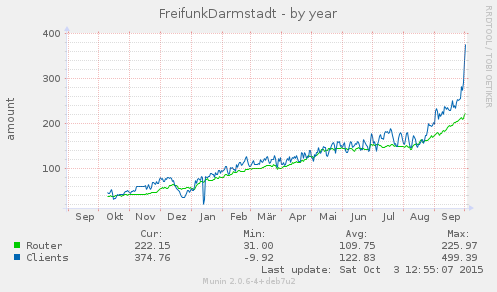
\includegraphics[width=0.8\textwidth]{images/ffda-Okt14-15}
      \end{center}
    \end{frame}

    \begin{frame}{1.x Jahre Freifunk Darmstadt}
      \vfill
      \begin{itemize}
        \item Oktober 2015: 230 Knoten - 600 gleichzeitige Nutzer
        \item Heute: 350 Knoten, 1000 gleichzeitige Nutzer
        % online nodes: https://api.darmstadt.freifunk.net/alfred/nodeinfo-statistics.json
        % all nodes: https://map.darmstadt.freifunk.net/data/nodes.json
      \end{itemize}
      \begin{center}
        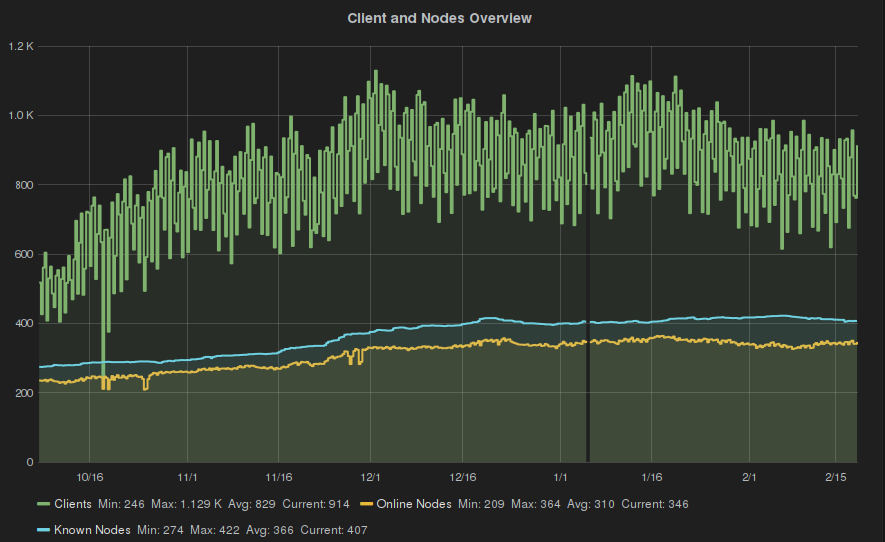
\includegraphics[width=0.8\textwidth]{images/ffda-Okt15-Feb16}
      \end{center}
    \end{frame}

    \begin{frame}{Stand September 2014}
      ca. 30 Knoten
      \begin{center}
        \vfill
        \begin{center}
          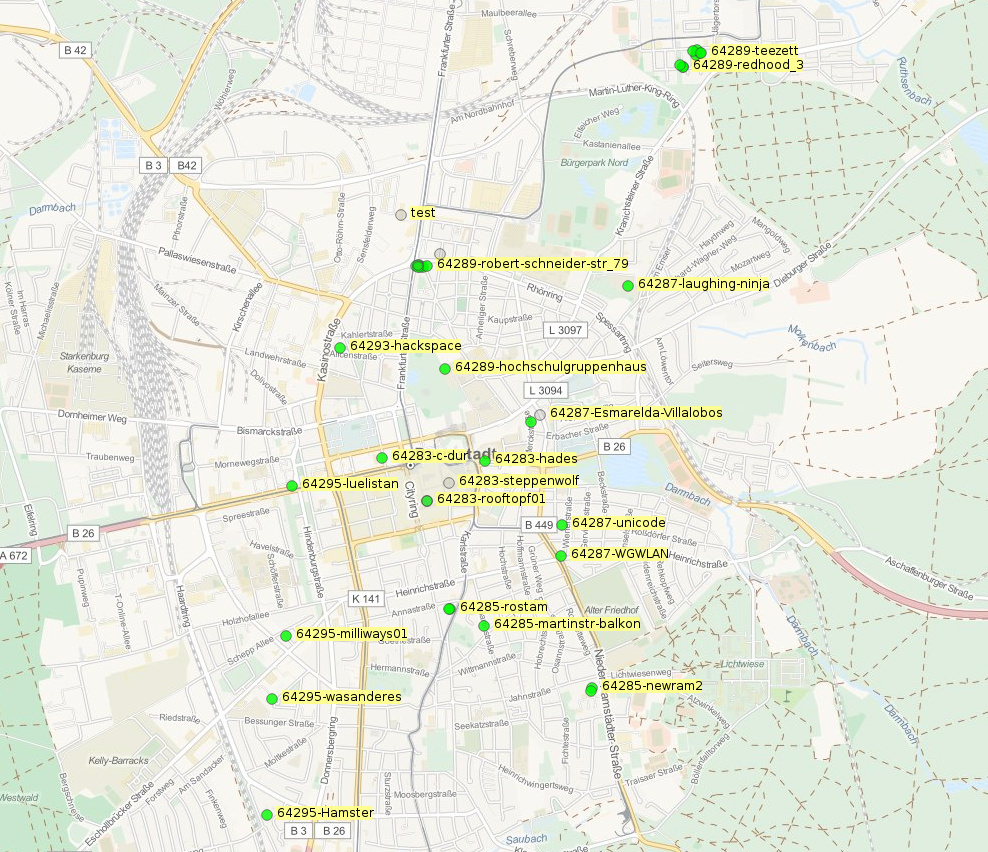
\includegraphics[height=6.5cm]{images/darmstadt-map}
        \end{center}
        \vfill
        \url{https://map.darmstadt.freifunk.net}
      \end{center}
    \end{frame}

    \begin{frame}{Stand Februar 2016}
      350 Knoten mit täglich über 1000 gleichzeitig aktiven Nutzern
      \begin{center}
        \vfill
        \begin{center}
          \only<1>{
            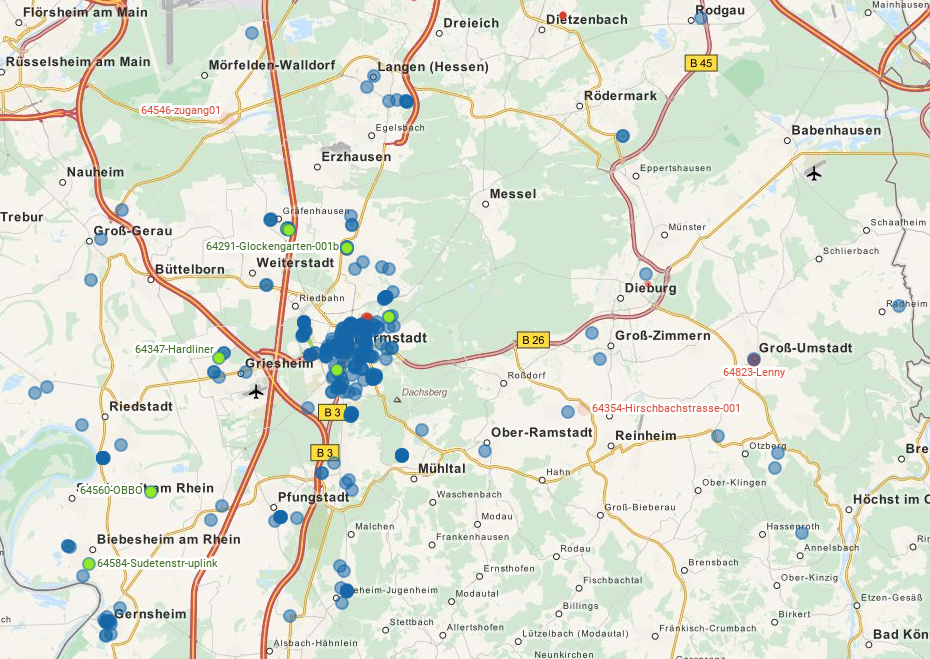
\includegraphics[height=6.5cm]{images/2016-02-17_map-large}
          }
          \only<2>{
            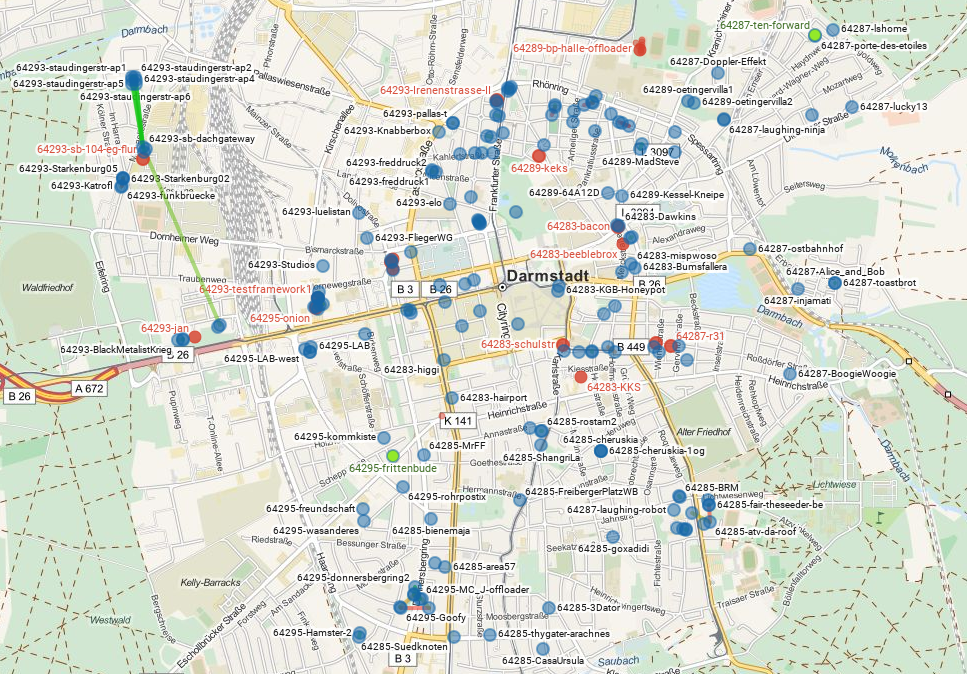
\includegraphics[height=6.5cm]{images/2016-02-17_map-darmstadt}
          }
        \end{center}
        \vfill
        \url{https://map.darmstadt.freifunk.net}
      \end{center}
    \end{frame}

  \section{Aktuelle Aufgaben}

    \begin{frame}{Aktuelle Aufgaben}
      \begin{columns}[T]
        \begin{column}{5cm}
          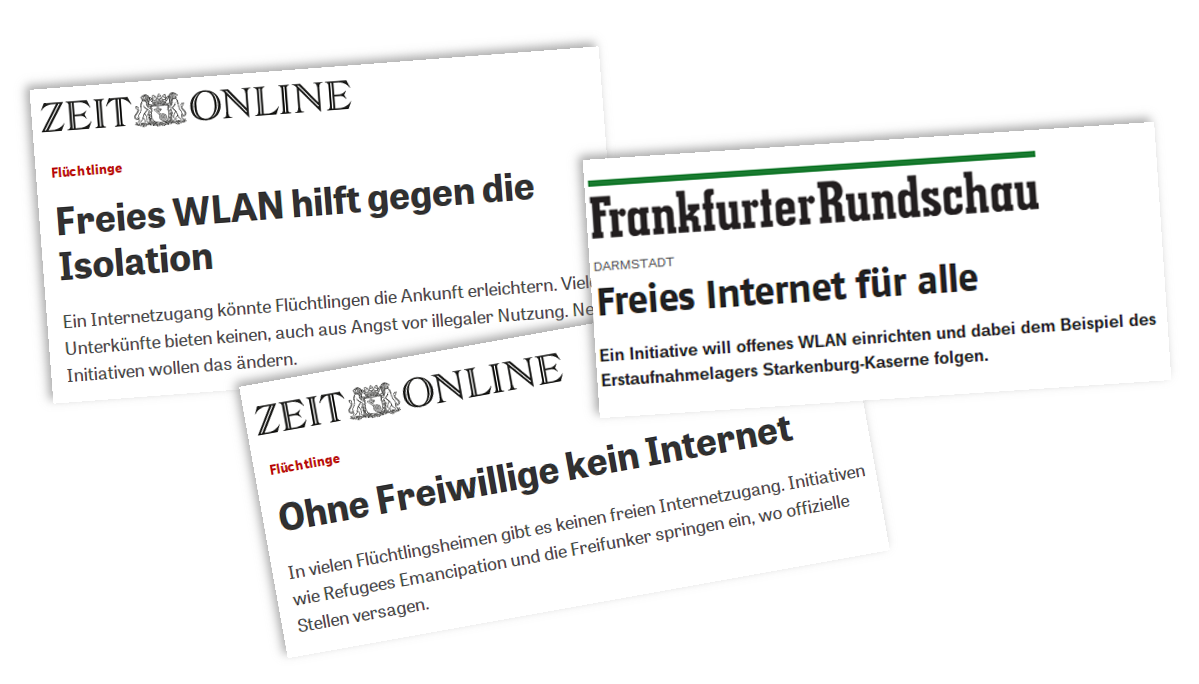
\includegraphics[width=\textwidth]{images/2015-10_presse-fluechtlinge}
          \vspace{1em}
          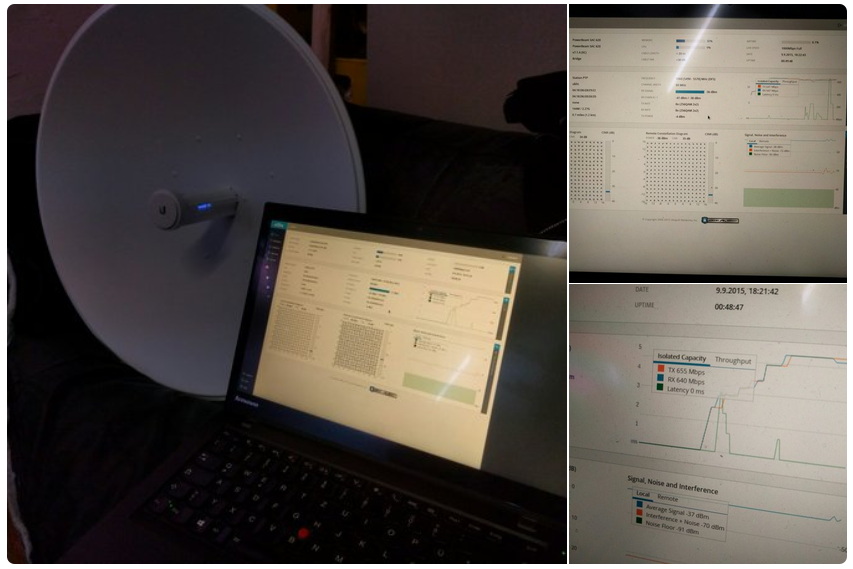
\includegraphics[width=\textwidth]{images/powerbeam-mit-laptop}
        \end{column}
        \begin{column}{7cm}
        \begin{itemize}
          \item \large \textbf{Flüchtlingsunterkünfte} mit Internet versorgen
          \item Freifunk-\textbf{Software} weiterentwickeln
          \item \textbf{Unterstützer} gewinnen
          \item \textbf{Öffentliche Plätze} versorgen
          \item Verbindungen zu \textbf{anderen Communities} aufbauen (ICVPN, Richtfunk)
          \item Wireless-\textbf{Backbone}
        \end{itemize}
        \end{column}
      \end{columns}

    \end{frame}

    \begin{frame}{Fragen? $\Rightarrow$ Foyer}
      \vfill
      \centering
      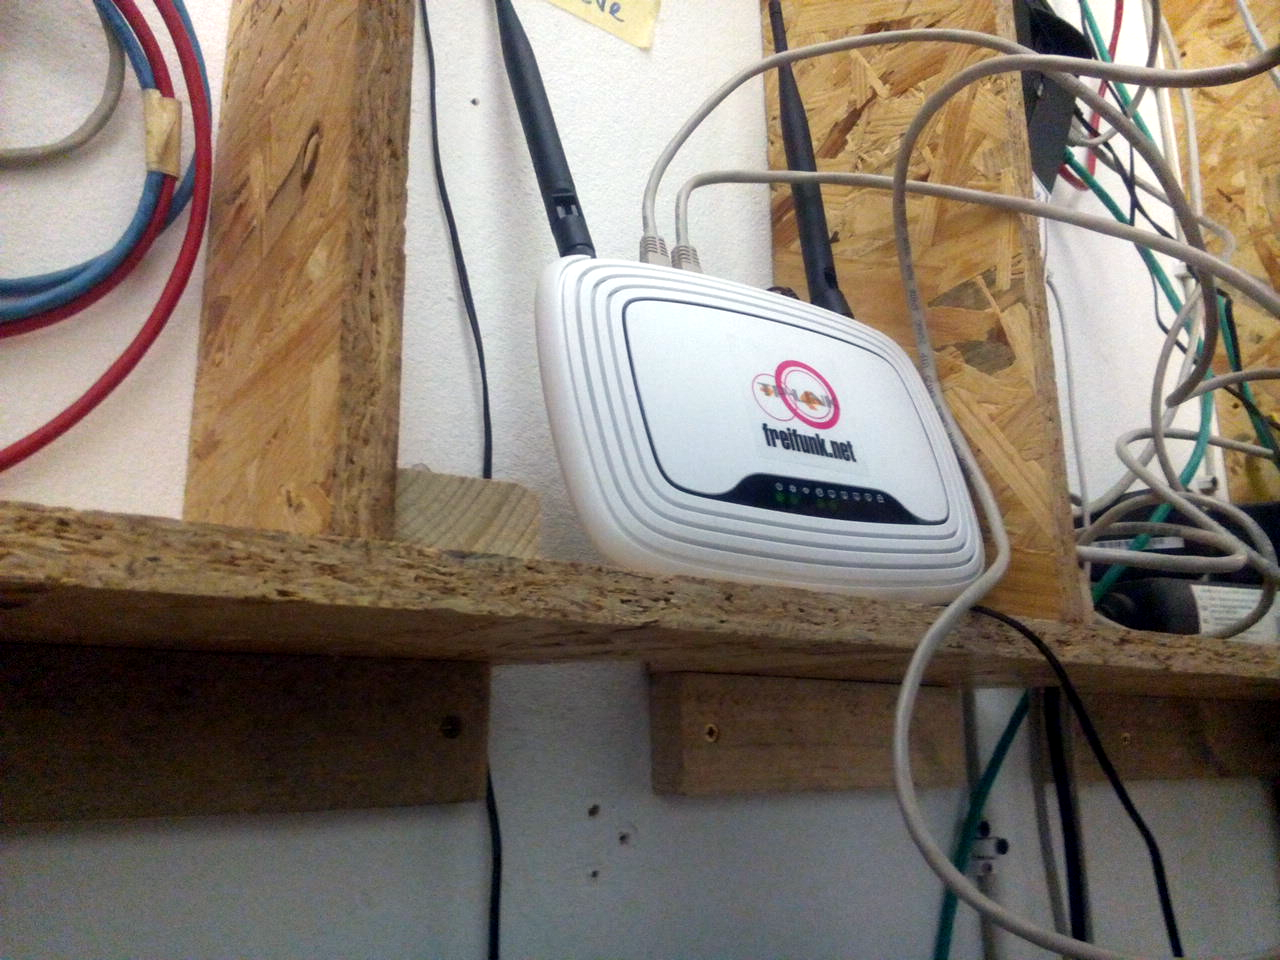
\includegraphics[width=0.7\textwidth]{images/irl_router}
      \vfill
    \end{frame}

\end{document}
